\documentclass[11pt]{article}

\usepackage[margin=0.85in]{geometry}
\usepackage[T1]{fontenc}
\usepackage[utf8]{inputenc}
\usepackage{lmodern}
\usepackage{microtype}
\usepackage{graphicx}
\usepackage{booktabs}
\usepackage{array}
\usepackage{amsmath}
\usepackage{amssymb}
\usepackage{hyperref}
\usepackage{xcolor}
\usepackage{caption}
\usepackage{subcaption}
\usepackage{float}

\hypersetup{
  colorlinks=true,
  linkcolor=blue,
  citecolor=blue,
  urlcolor=blue
}

\newcommand{\outputroot}{/home/lachlan/ProjectsLFS/OrganoidAgent/analysis-outputs/yichao_future_expression}

\title{\textbf{Negative Result Report: Brightfield-to-Fluorescence Feasibility Does Not Transfer to Reliable Future Expression Prediction}}
\author{OrganoidAgent Yichao analysis}
\date{May 11, 2026}

\begin{document}
\maketitle

\begin{abstract}
This report documents the completed Yichao projected-organoid prediction experiments with an explicit negative-result interpretation. Same-time brightfield-to-fluorescence prediction ($B_t \rightarrow F_t$) is feasible: the held-out test set achieved image MAE 0.1077, positive AUROC 0.728, and fluorescence peak Pearson correlation 0.685. However, future fluorescence prediction from earlier brightfield ($B_{0:k} \rightarrow F_{p>k}$) is not solved by the current models. The scalar future model achieved only AUROC 0.228 and future peak Pearson 0.134. The joint model, despite combining same-time B2F supervision and dense future fluorescence prediction, achieved AUROC 0.223 and future peak Pearson -0.049 on the held-out test split. Visual outputs confirm the problem: predicted future fluorescence is not close to the true future fluorescence. The correct conclusion is that the current data/track/target design supports same-time morphology-to-fluorescence feasibility, but does not yet support robust early future expression prediction.
\end{abstract}

\section{Purpose}

The goal was to test four progressively harder questions:

\begin{enumerate}
\item Can projected brightfield predict contemporaneous fluorescence?
\item Which explicit organoid morphology features explain fluorescence distinction?
\item Can early brightfield predict later fluorescence expression?
\item Can a joint model use same-time B2F as auxiliary supervision to improve future prediction?
\end{enumerate}

Only the first two questions currently have a positive answer. The future-prediction questions produced negative results on held-out test data.

\section{Data and Splits}

The projected complete/non-edge Yichao dataset was built from:

\begin{center}
\small
\path{\outputroot/future_expression.sqlite}
\end{center}

The prepared dataset contains 9,380 projected complete/non-edge organoid instances, 363 linked time-series tracks, and 6,088 early-prefix future samples. The future samples are split into 4,277 train, 1,178 validation, and 633 held-out test samples.

\section{Model Tasks}

\subsection{Same-time B2F}

The same-time model learns:
\begin{equation}
  \hat{F}_t = G_\theta(B_t),
\end{equation}
where $B_t$ is the projected brightfield crop and $F_t$ is the corresponding projected fluorescence crop.

The image loss uses organoid masks:
\begin{equation}
\mathcal{L}_{\mathrm{img}} =
\mathrm{mean}(|\hat{F}-F|M)
+0.2\mathrm{mean}(|\hat{F}-F|(1-M)).
\end{equation}

\subsection{Scalar future baseline}

The scalar future model takes a brightfield prefix and morphology features:
\begin{equation}
P_k = \{(B_j, X_j)\}_{j=k-L+1}^{k},
\end{equation}
and predicts future-positive status, future peak fluorescence, and future fluorescence AUC:
\begin{equation}
(\hat{a}_p,\hat{r}_p,\hat{q}_p) = H_\phi(P_k), \quad p > k.
\end{equation}

\subsection{Joint future model}

The joint model adds dense image supervision:
\begin{equation}
(\hat{F}_p,\hat{a}_p,\hat{r}_p,\hat{q}_p,\hat{F}_k)
= J_\psi(P_k, B_k),
\end{equation}
with objective:
\begin{equation}
\mathcal{L}
= \mathcal{L}_{\mathrm{img}}(\hat{F}_p,F_p,M_p)
+0.5\mathcal{L}_{\mathrm{img}}(\hat{F}_k,F_k,M_k)
+0.25\mathcal{L}_{\mathrm{scalar}}.
\end{equation}

The intended intuition was reasonable: because $B_t \rightarrow F_t$ is learnable, auxiliary B2F might regularize the representation used for $B_{0:k} \rightarrow F_p$. The held-out test result shows that this was not enough.

\section{Quantitative Results}

\begin{table}[H]
\centering
\caption{Final held-out test metrics. The B2F task works; both future-prediction tasks fail to generalize.}
\begin{tabular}{lccc}
\toprule
Metric & Same-time B2F & Scalar future & Joint future \\
\midrule
Test examples & 1,088 & 633 & 633 \\
Positive examples & 14 & not recorded in metric JSON & 11 \\
Image MAE & 0.1077 & not predicted & 0.3112 \\
Image PSNR & 14.18 dB & not predicted & 7.95 dB \\
Positive AUROC & 0.728 & 0.228 & 0.223 \\
Average precision & 0.110 & 0.0156 & 0.0127 \\
Peak Pearson & 0.685 & 0.134 & -0.049 \\
AUC Pearson & not applicable & 0.105 & 0.075 \\
\bottomrule
\end{tabular}
\end{table}

\paragraph{Interpretation.}
The future classifiers are worse than useful random-ranking baselines on the held-out test set. The joint model's dense future fluorescence prediction also fails visually and quantitatively: image MAE is high, PSNR is low, and the prediction panels show outputs that do not match the true future fluorescence.

\section{Same-Time B2F Is Feasible}

\begin{figure}[H]
\centering
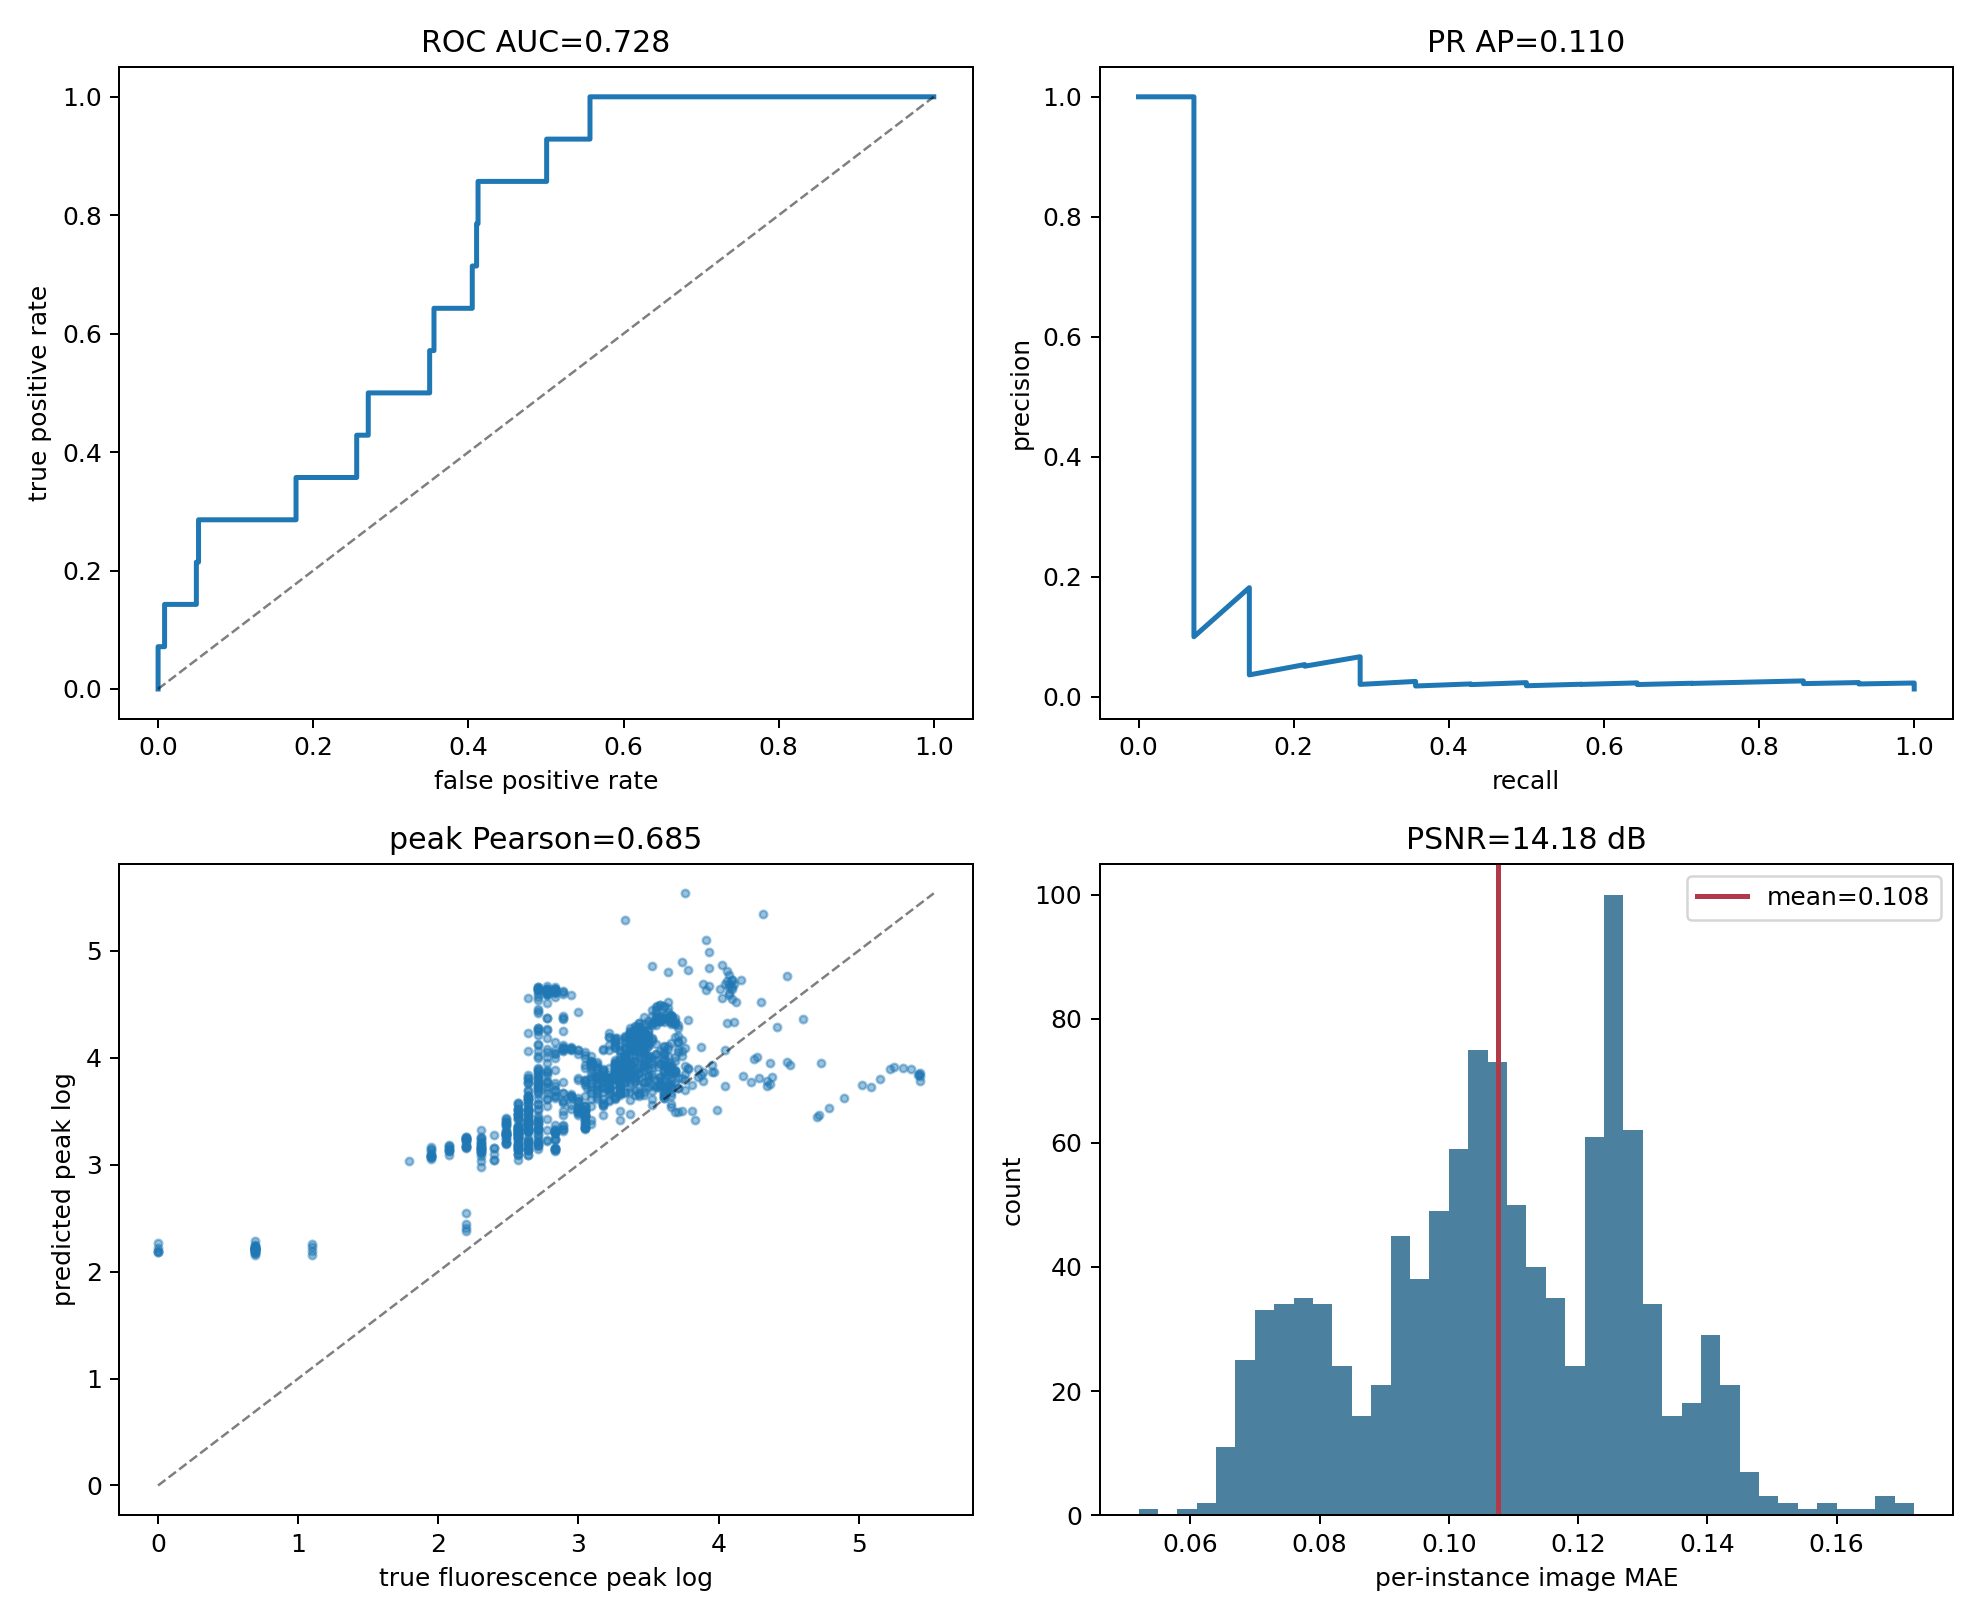
\includegraphics[width=\linewidth]{figures/fig1_b2f_performance_summary.png}
\caption{Same-time B2F performance summary. This is the positive part of the experiment: the predicted fluorescence intensity has meaningful held-out correlation with true fluorescence.}
\label{fig:b2f-summary}
\end{figure}

\begin{figure}[H]
\centering
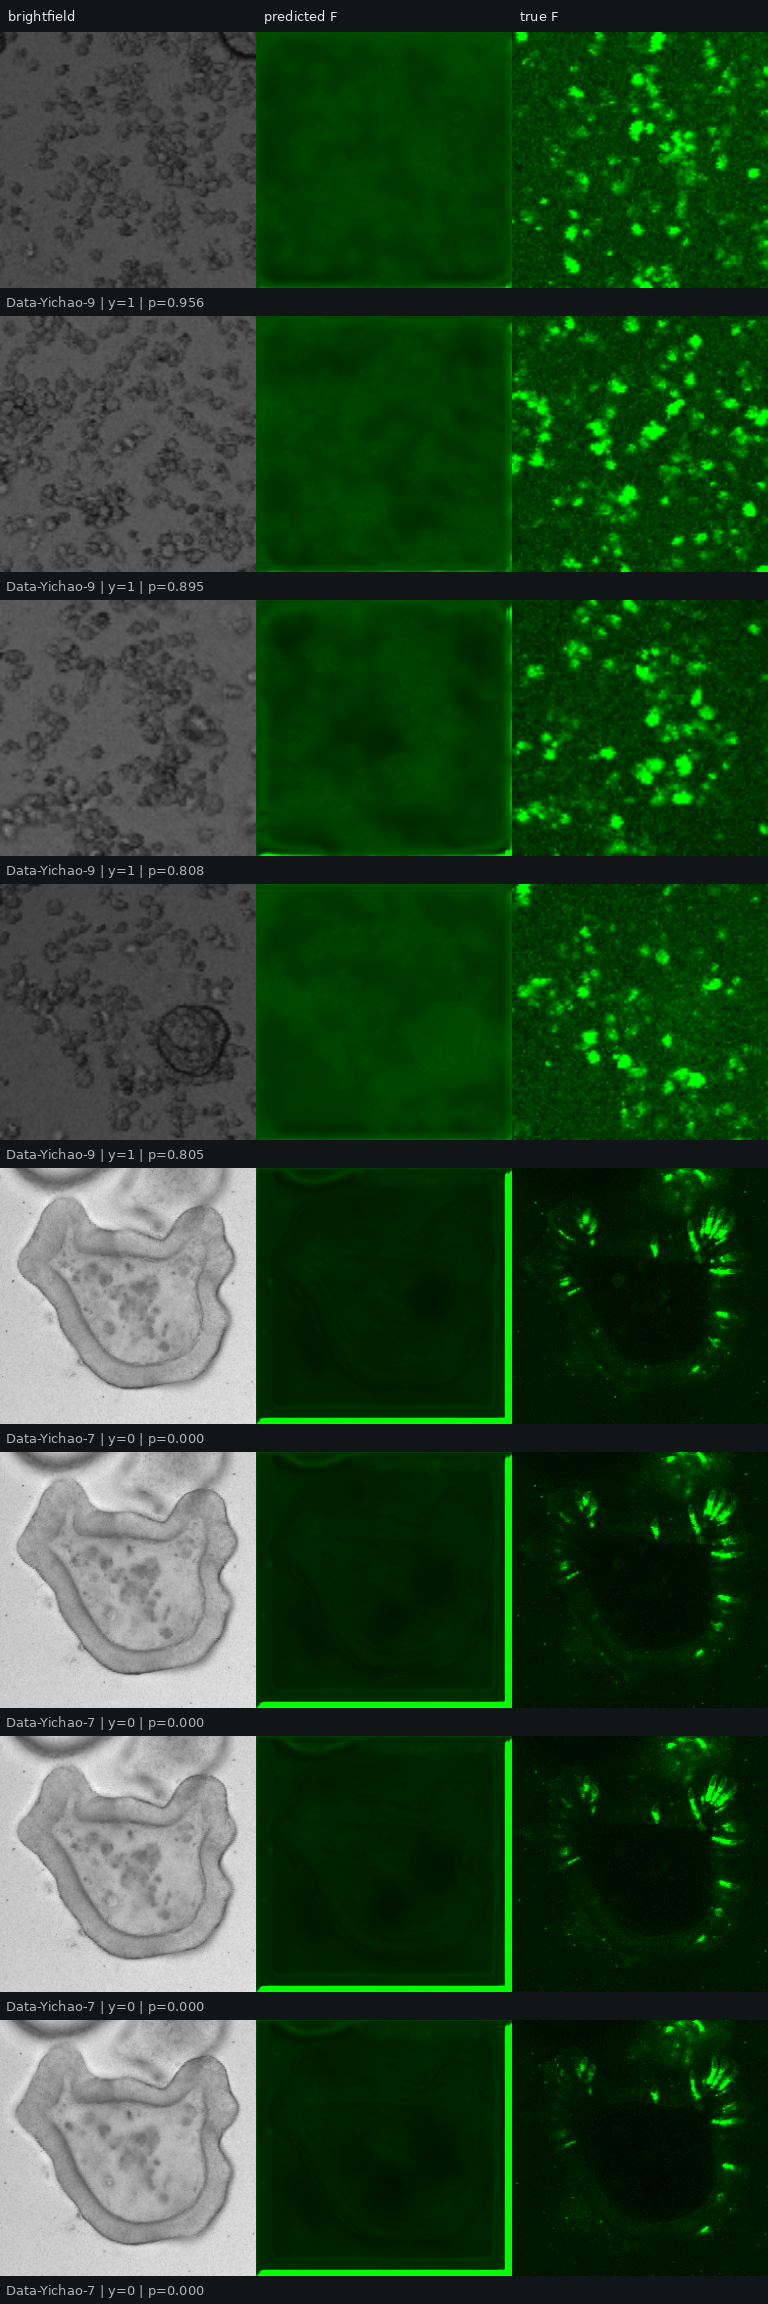
\includegraphics[height=0.82\textheight,keepaspectratio]{figures/fig2_b2f_predictions.png}
\caption{Held-out same-time B2F prediction examples. Columns show brightfield input, predicted fluorescence, and true fluorescence.}
\label{fig:b2f-examples}
\end{figure}

The B2F result establishes that brightfield morphology contains contemporaneous fluorescence-related information. This does not imply that early brightfield contains enough information to predict future expression.

\section{Feature Explanation}

\begin{figure}[H]
\centering
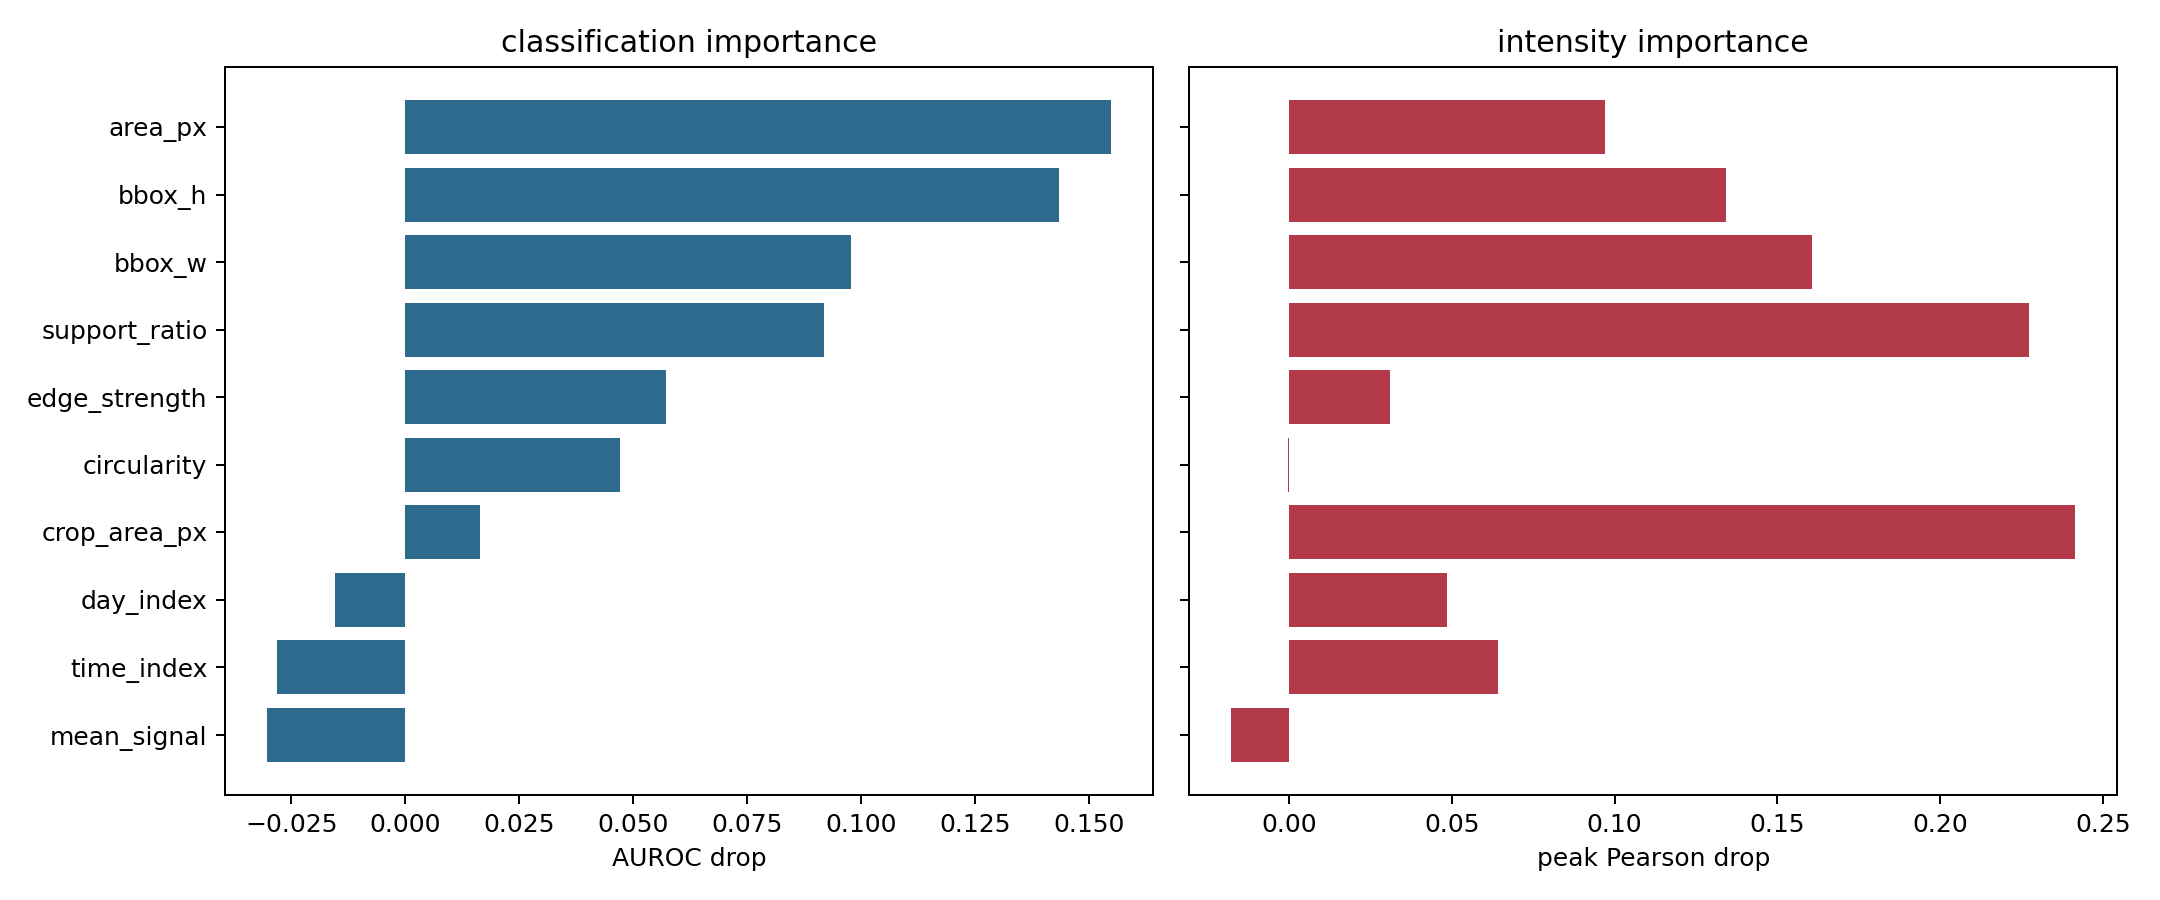
\includegraphics[width=0.92\linewidth]{figures/fig3_feature_importance.png}
\caption{Explicit feature explanation for fluorescence distinction. Size and morphology features are the strongest signals.}
\label{fig:feature-importance}
\end{figure}

\begin{table}[H]
\centering
\caption{Top explanatory features from same-time feature analysis.}
\begin{tabular}{lcc}
\toprule
Feature & AUROC drop & Peak-correlation drop \\
\midrule
Area & 0.155 & 0.097 \\
Bounding-box height & 0.143 & 0.134 \\
Bounding-box width & 0.098 & 0.161 \\
Support ratio & 0.092 & 0.227 \\
Edge strength & 0.057 & 0.031 \\
Circularity & 0.047 & -0.000 \\
\bottomrule
\end{tabular}
\end{table}

These features are plausible and useful for same-time fluorescence distinction. They mainly describe organoid size, projected shape, segmentation support, and boundary quality. They are not sufficient evidence that future differentiation can be predicted before expression.

\section{Scalar Future Prediction Fails}

\begin{figure}[H]
\centering
\begin{subfigure}[b]{0.49\linewidth}
\centering
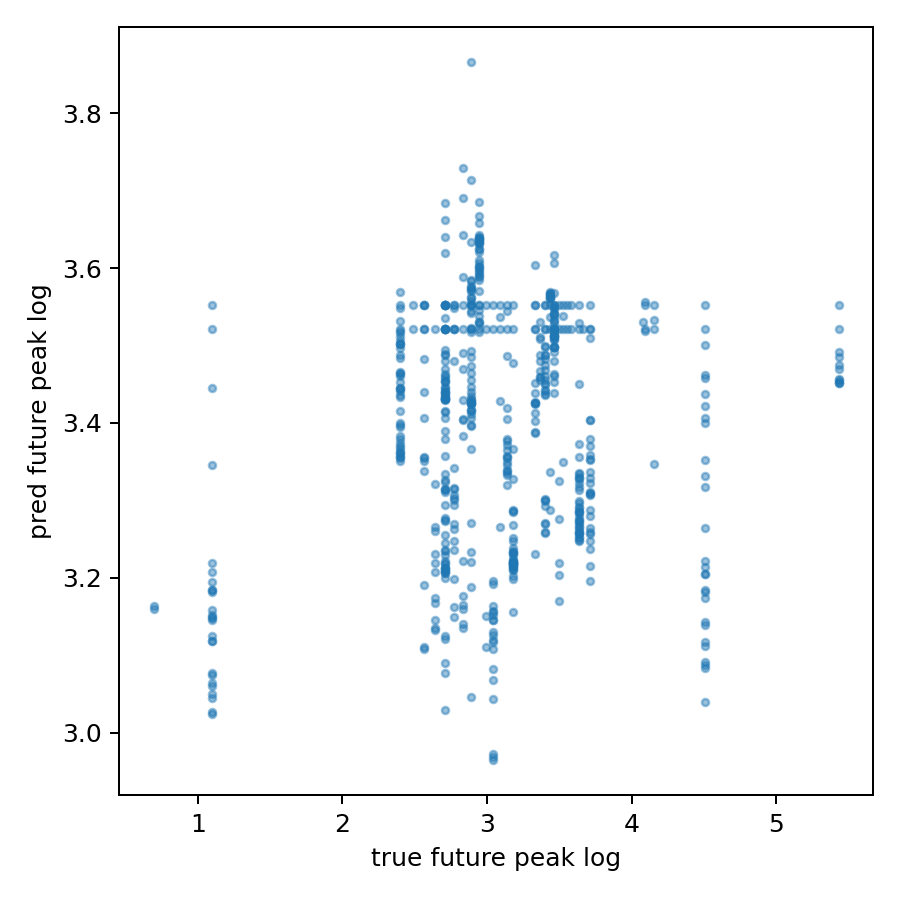
\includegraphics[width=\linewidth]{figures/fig4_scalar_future_peak_scatter.png}
\caption{Future peak prediction}
\end{subfigure}
\hfill
\begin{subfigure}[b]{0.49\linewidth}
\centering
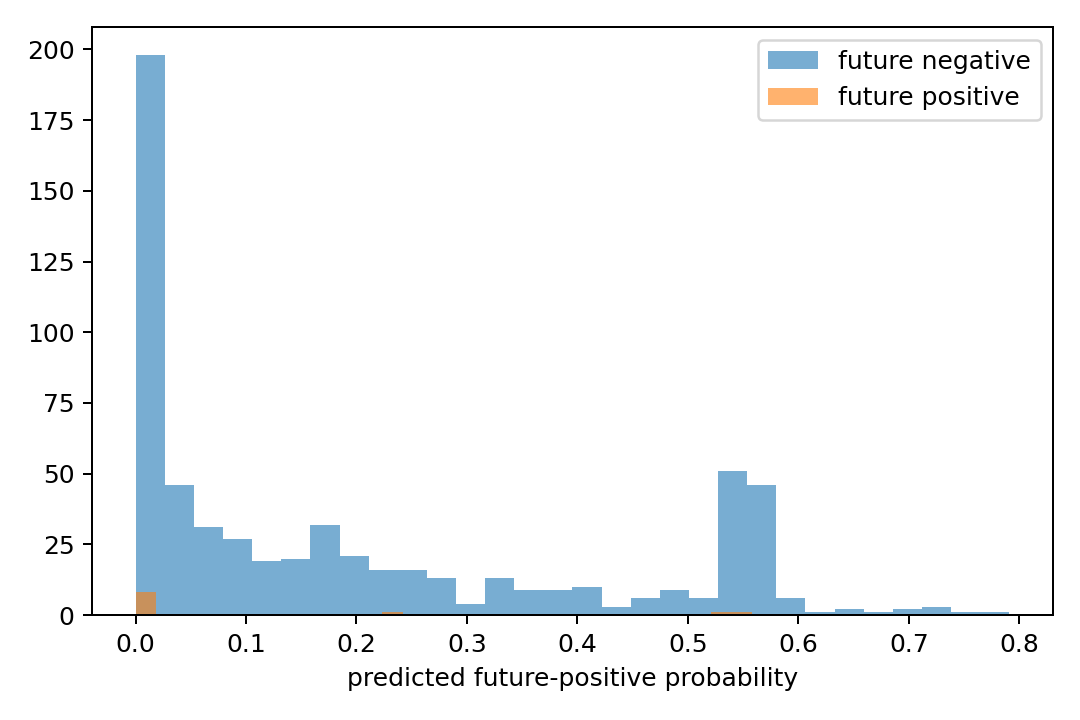
\includegraphics[width=\linewidth]{figures/fig5_scalar_future_score_histogram.png}
\caption{Future-positive score distribution}
\end{subfigure}
\caption{Scalar future baseline outputs. The prediction is not close enough to truth for useful future expression prediction.}
\label{fig:scalar-future}
\end{figure}

The scalar future model is essentially a negative baseline. It does not separate future-positive from future-negative examples and it does not predict the future fluorescence peak accurately enough to support biological inference.

\section{Joint Future Prediction Also Fails}

\begin{figure}[H]
\centering
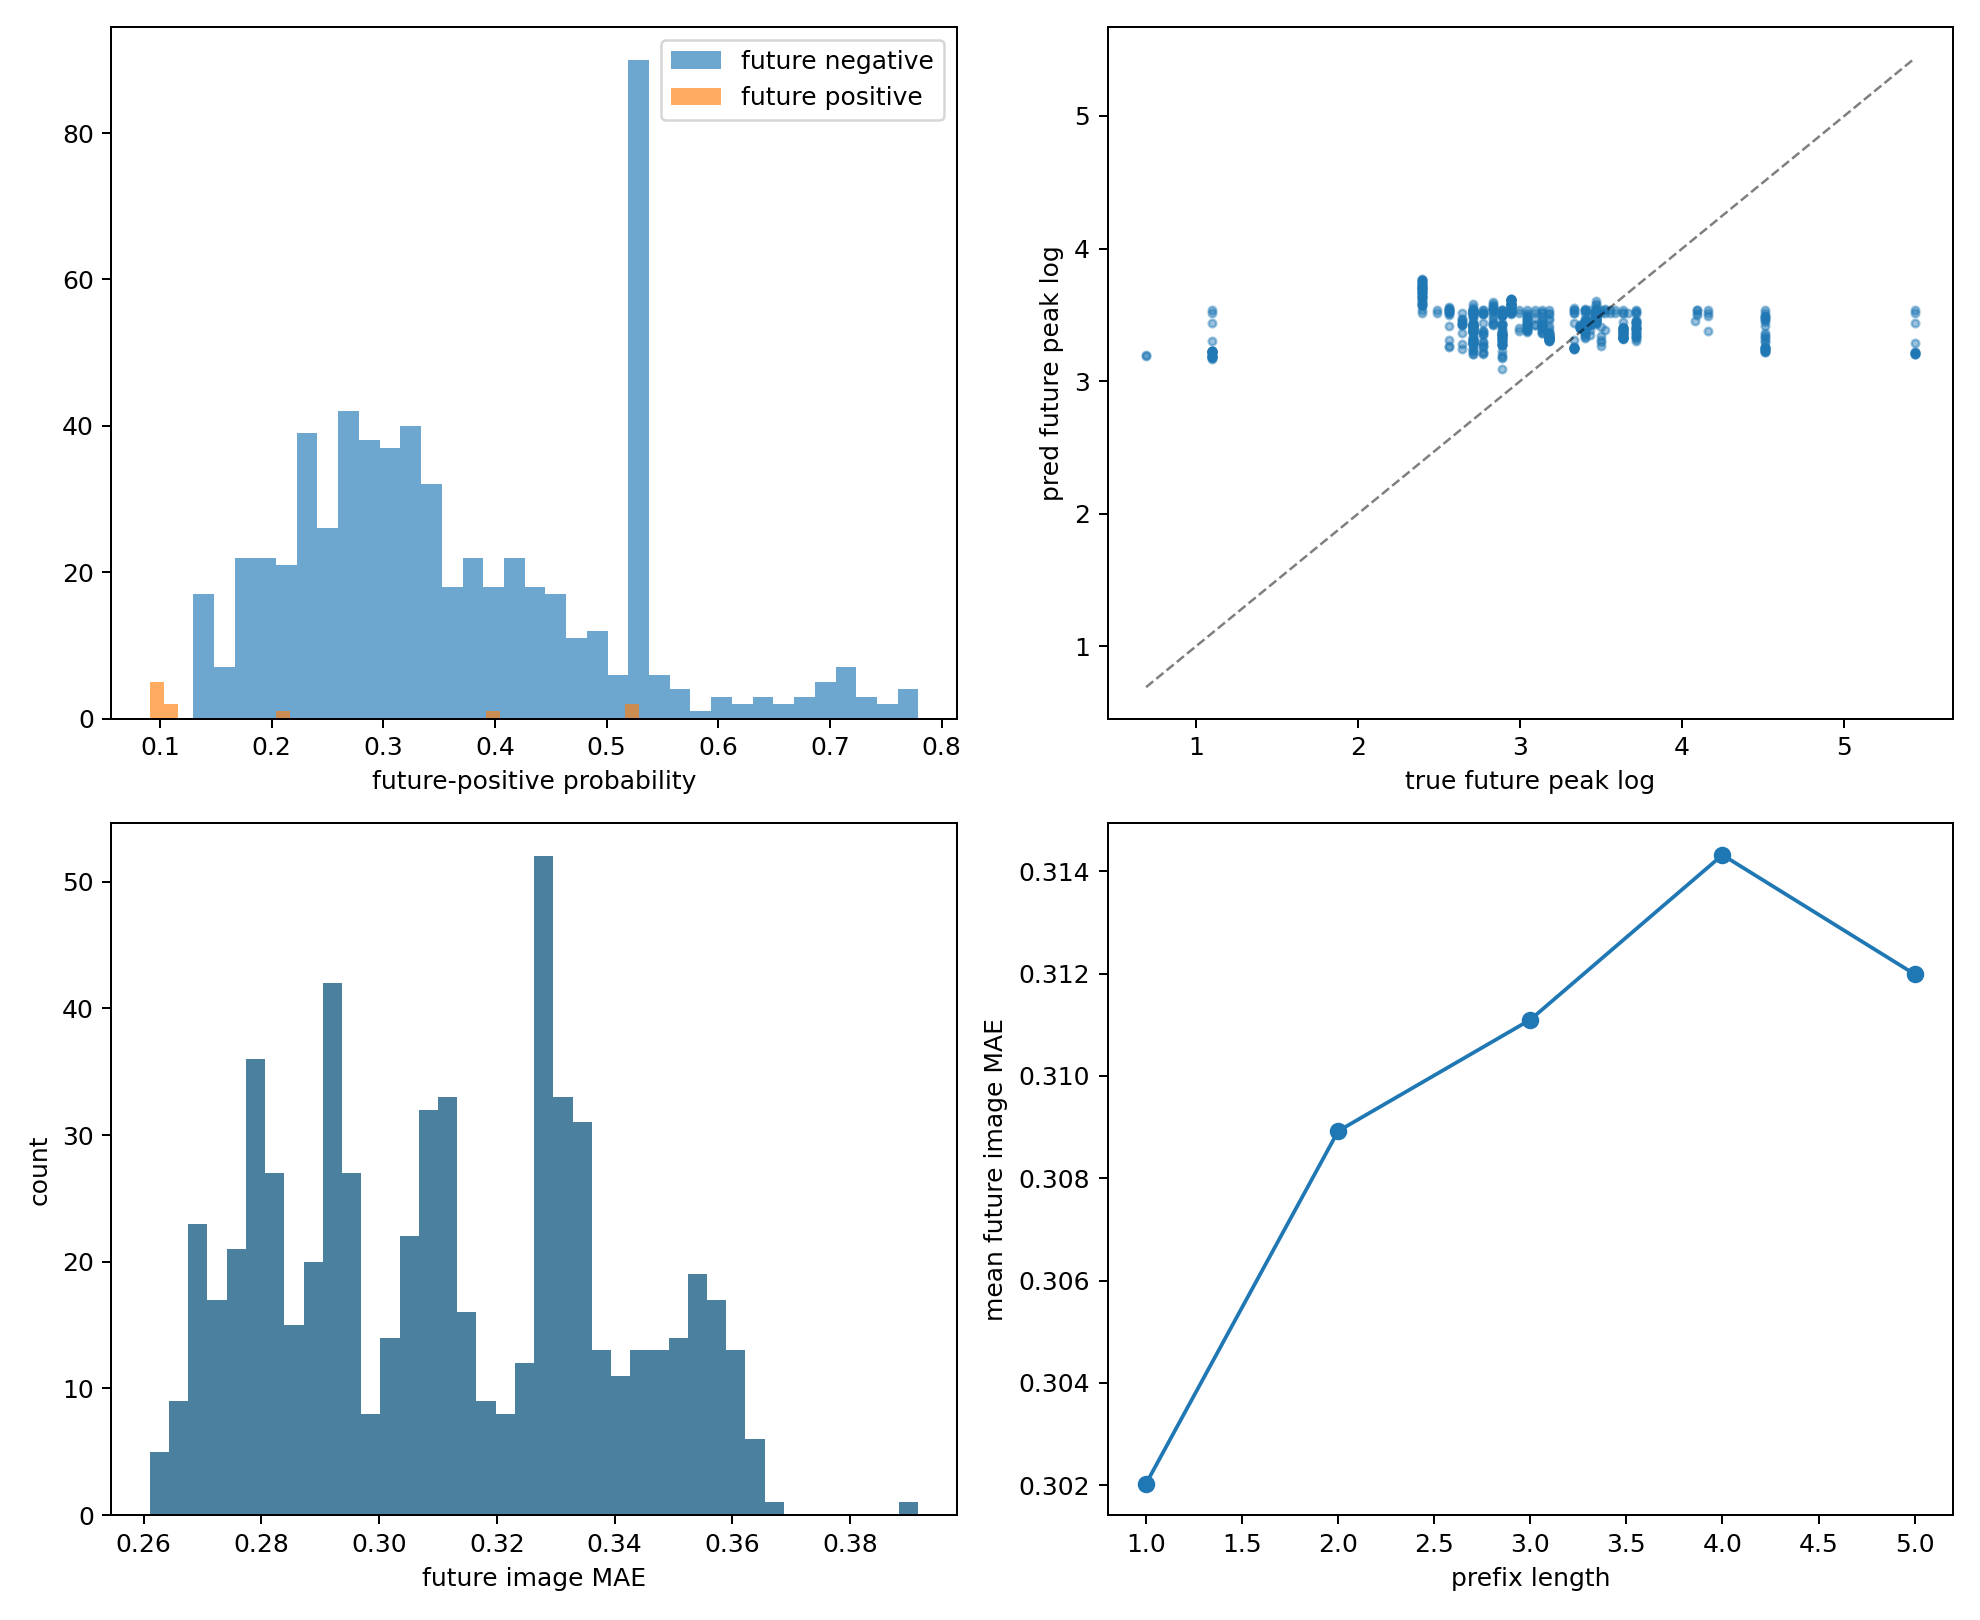
\includegraphics[width=\linewidth]{figures/fig7_joint_summary.png}
\caption{Joint model final test summary. Validation appeared promising during training, but the selected model does not generalize on the held-out future test split.}
\label{fig:joint-summary}
\end{figure}

\begin{figure}[H]
\centering
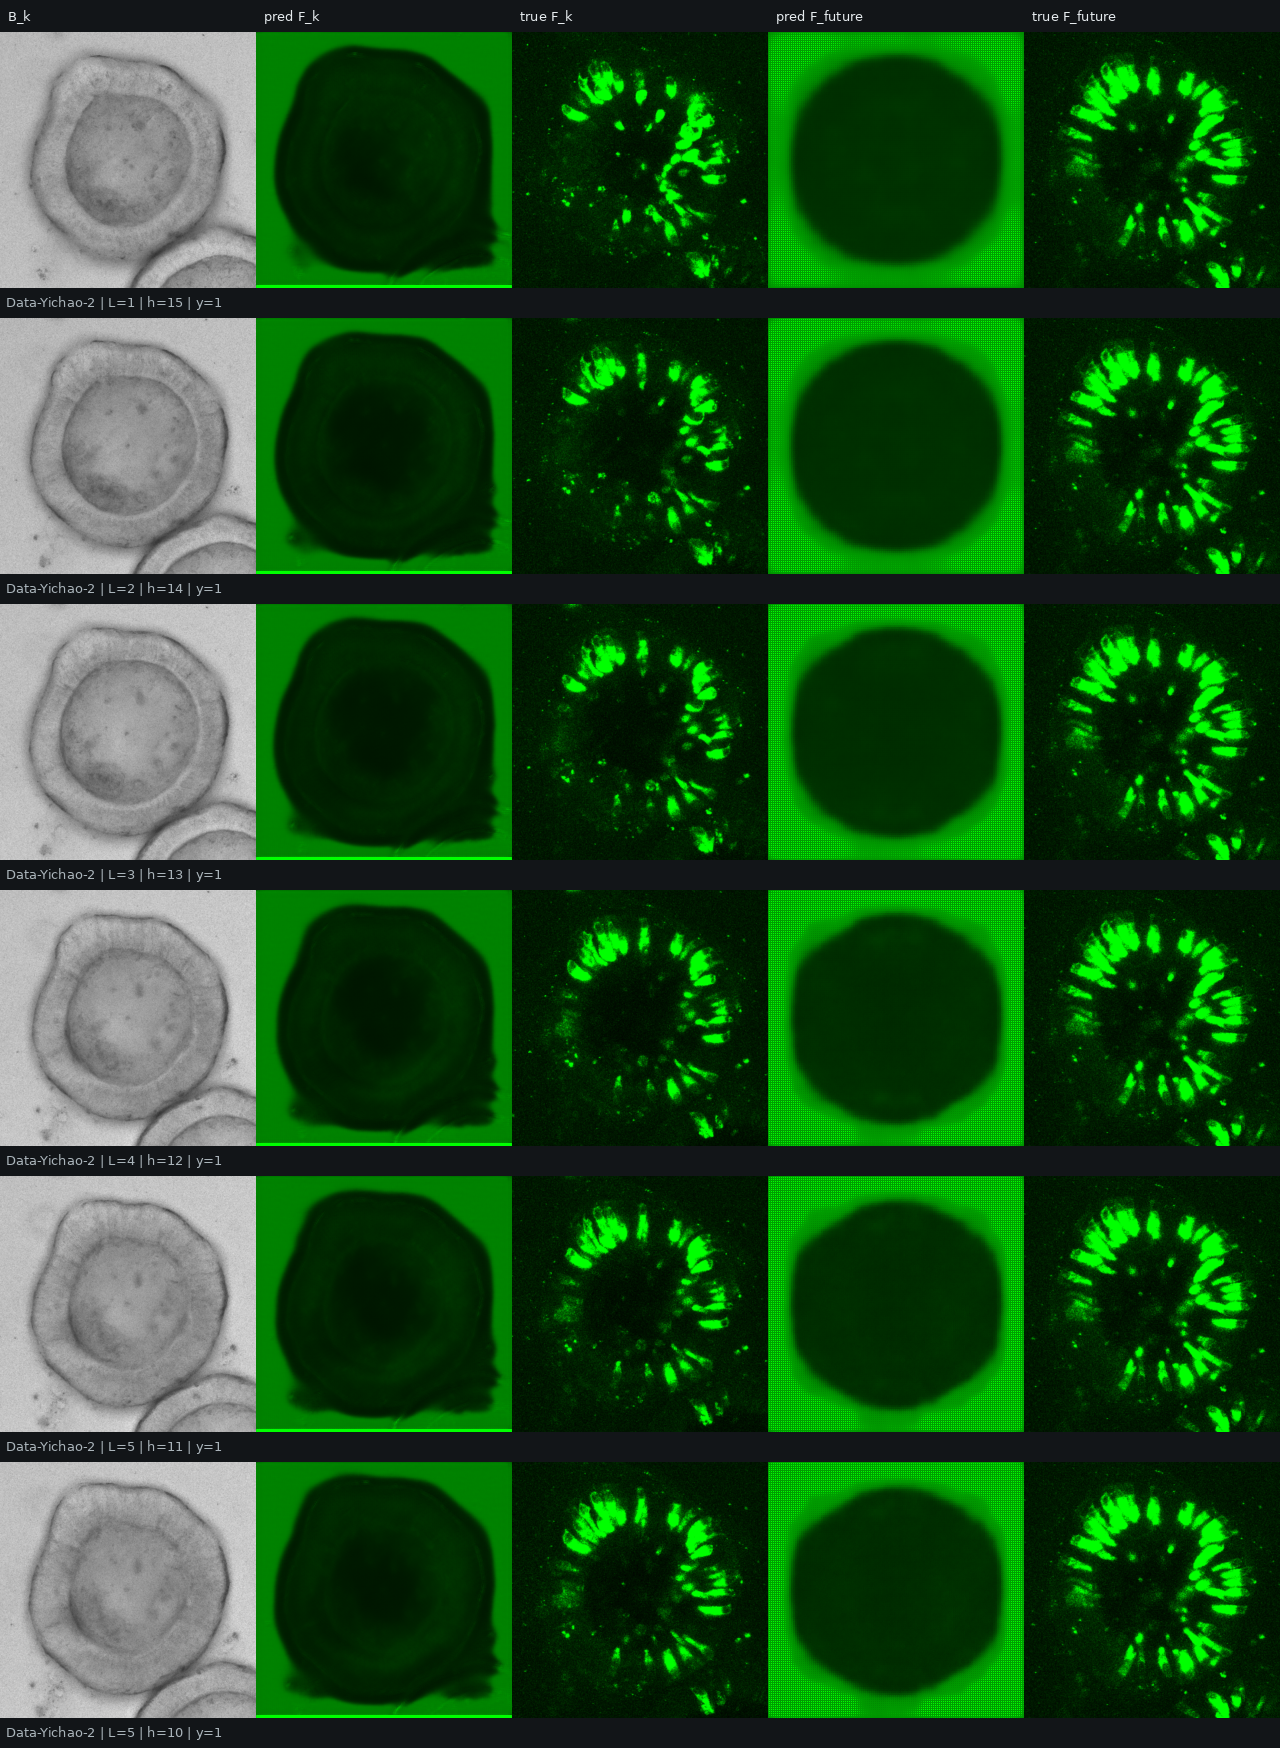
\includegraphics[height=0.82\textheight,keepaspectratio]{figures/fig6_joint_test_predictions.png}
\caption{Joint model held-out test prediction panel. Columns show current brightfield, predicted current fluorescence, true current fluorescence, predicted future fluorescence, and true future fluorescence. This panel is the most direct visual evidence that the future prediction is not close to the truth.}
\label{fig:joint-predictions}
\end{figure}

\begin{figure}[H]
\centering
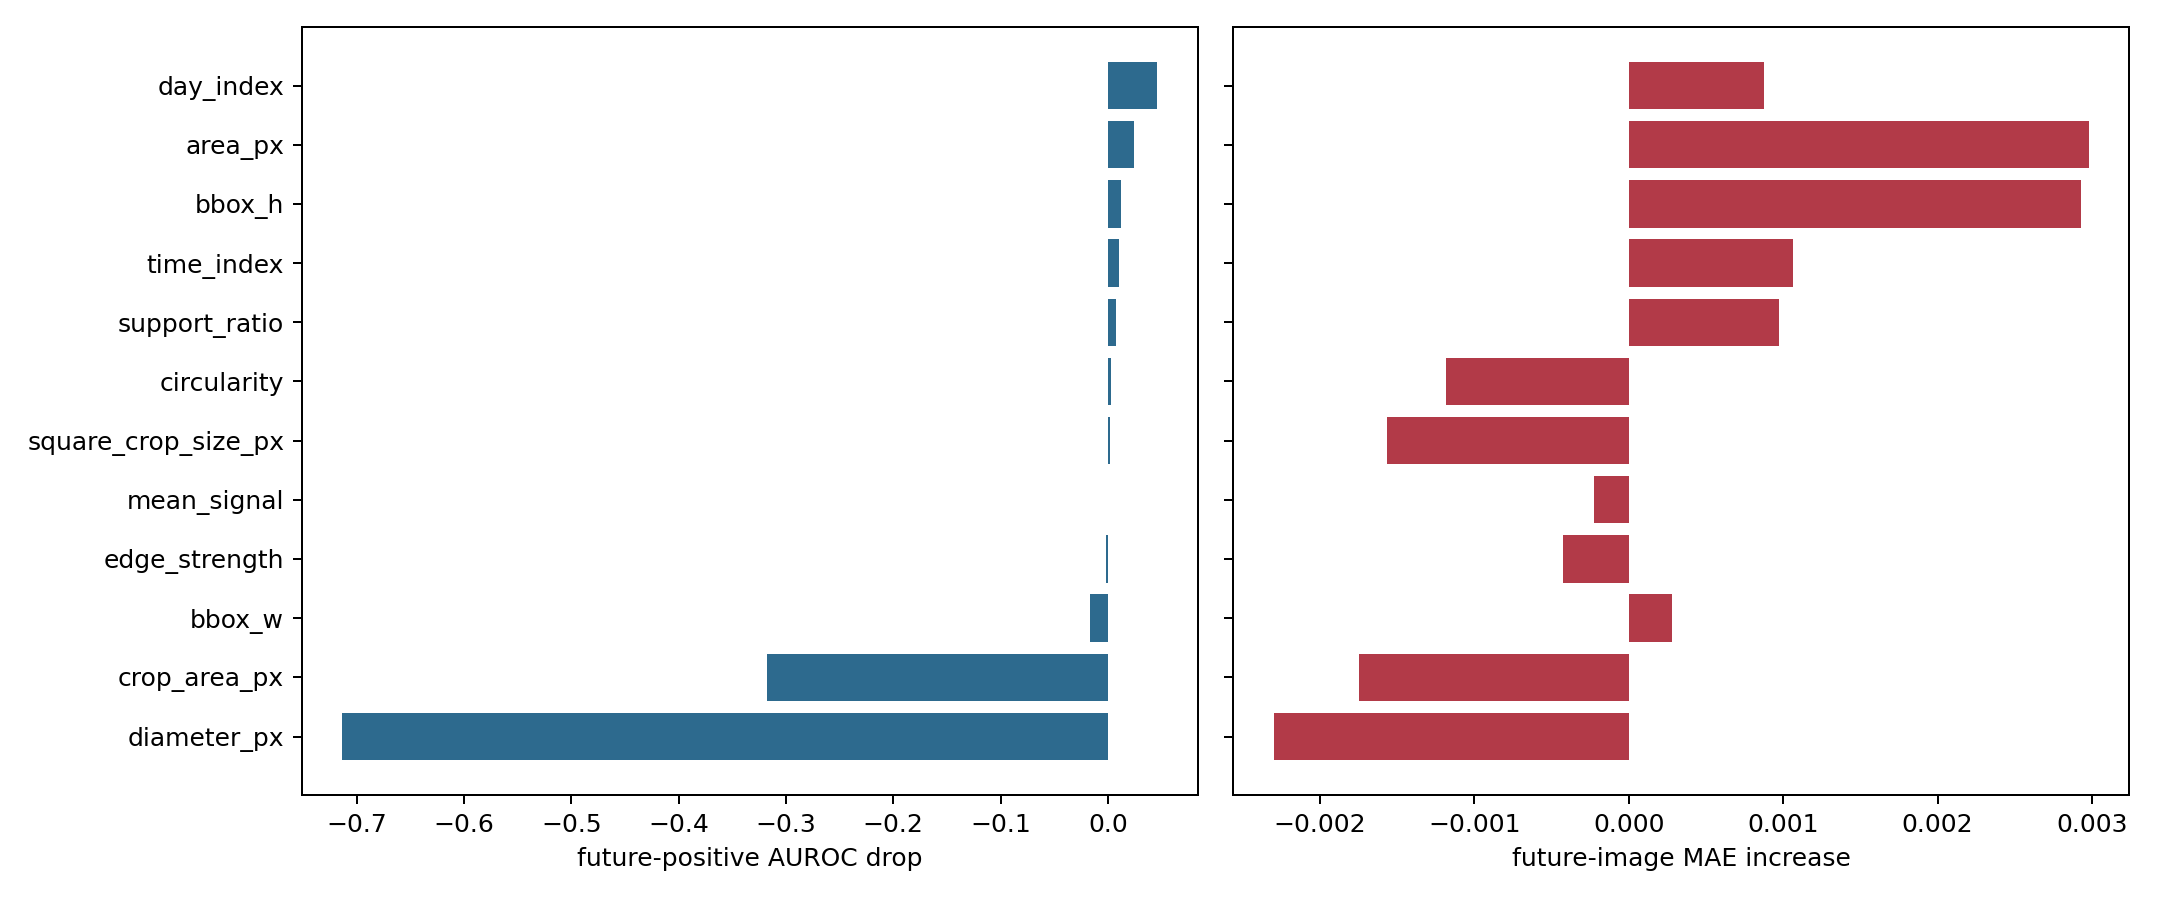
\includegraphics[width=0.92\linewidth]{figures/fig8_joint_feature_ablation.png}
\caption{Joint model feature ablation. Some temporal/size features affect the weak classifier, but the overall held-out future prediction remains poor.}
\label{fig:joint-ablation}
\end{figure}

The joint model did not rescue the future task. The most important observation is not just the weak scalar metrics, but the visual mismatch in Fig.~\ref{fig:joint-predictions}: the predicted future fluorescence is not close to the true future fluorescence.

\section{Likely Failure Causes}

The current negative result is technically useful. It narrows the problem:

\begin{enumerate}
\item \textbf{Same-time signal exists, but future signal may not be present early enough.} B2F learns $B_t \rightarrow F_t$, but this does not guarantee $B_{0:k} \rightarrow F_p$.
\item \textbf{Future-positive examples are rare.} The held-out joint test split has only 11 future-positive examples.
\item \textbf{Track linking is approximate.} Any wrong organoid association across time directly corrupts future targets.
\item \textbf{Last-frame target may be a poor biological endpoint.} The last available future frame may not equal the biologically most informative or peak-expression frame.
\item \textbf{Dataset/domain split effects are strong.} Validation performance looked better than held-out test performance, indicating nontrivial distribution shift.
\end{enumerate}

\section{Recommended Next Step}

Do not increase model complexity first. The next scientifically realistic step is to improve the data target:

\begin{enumerate}
\item Manually verify a subset of linked tracks, especially positive trajectories.
\item Train/evaluate by horizon: short future, medium future, long future.
\item Compare \texttt{last\_future} targets with \texttt{peak\_future} targets.
\item Build a cleaner positive-control dataset where Yichao confirms which structures are true positive cells versus debris/background.
\item Keep same-time B2F as a validated auxiliary or pretraining task, but do not claim future prediction yet.
\end{enumerate}

\section{Reproducibility}

Main completed output folders:

\begin{itemize}
\item Same-time B2F: \path{\outputroot/stage1_b2f_evaluation}
\item Scalar future baseline: \path{\outputroot/stage2_future_expression}
\item Joint future model: \path{\outputroot/stage3_joint_b2f_future}
\item Previous consolidated report: \path{\outputroot/previous_run_evaluation}
\end{itemize}

Main code folder:

\begin{center}
\small
\path{/home/lachlan/ProjectsLFS/OrganoidAgent/differentiation_prediction/yichao_future_expression}
\end{center}

\section{Conclusion}

The honest conclusion is:

\begin{quote}
The current Yichao projected dataset supports same-time brightfield-to-fluorescence prediction and morphology-based explanation, but it does not yet support reliable future fluorescence expression prediction from earlier brightfield. The separate and joint future models are negative results on held-out test data.
\end{quote}

This is still a useful result because it prevents overclaiming and clarifies the next experimental requirement: cleaner longitudinal tracking and positive-control future-expression targets.

\begin{thebibliography}{9}

\bibitem{isola2017pix2pix}
Isola, P., Zhu, J.-Y., Zhou, T. and Efros, A. A.
Image-to-image translation with conditional adversarial networks.
\textit{CVPR} (2017).
\url{https://arxiv.org/abs/1611.07004}

\bibitem{fnet}
Allen Cell Modeling.
Pytorch-FNet: label-free prediction of fluorescence images from transmitted-light microscopy.
\url{https://allencellmodeling.github.io/pytorch_fnet/}

\bibitem{vafaeikia2020}
Vafaeikia, P., Namdar, K. and Khalvati, F.
A brief review of deep multi-task learning and auxiliary task learning.
\url{https://arxiv.org/abs/2007.01126}

\end{thebibliography}

\end{document}
